\documentclass {beamer}

%
% Custom operator declarations
%
\DeclareMathOperator{\ZZ}{\mathbb{Z}}
\DeclareMathOperator{\CC}{\mathbb{C}}
\DeclareMathOperator{\hh}{\mathfrak{h}}
\DeclareMathOperator{\re}{\text{Re}}
\DeclareMathOperator{\im}{\text{Im}}



%
% Custom theme
%
\usetheme{AAUsimple}

\title{Algebro-Geometric Approach to Nonlinear Integrable Equations}
\subtitle{General Examination}
\author{
  Chris Swierczewski\\
  {\tt cswiercz@uw.edu}
}
\institute{
  Department of Applied Mathematics\\
  University of Washington\\
  Seattle, Washington
}
\pgfdeclareimage[height=1.5cm]{titlepagelogo}{AAUgraphics/aau_logo_new_circle}
\titlegraphic{
  \pgfuseimage{titlepagelogo}
}


% Ideas:

% o add a seriers of cartoons demonstrating the concept of
% homotopy. relate to integration.



%%%%%%%%%%%%%%%%%%%%%%%%%%%%%%%%%%%%%%%%%%%%%%%%%%%%%%%%%%%%%%%%%%%%%%%%%%%%%%%
\begin{document}
%%%%%%%%%%%%%%%%%%%%%%%%%%%%%%%%%%%%%%%%%%%%%%%%%%%%%%%%%%%%%%%%%%%%%%%%%%%%%%%

\begin{frame}[plain,noframenumbering]
  \titlepage
\end{frame}

\begin{frame}{Table of Contents}{}
  \tableofcontents
\end{frame}

%%%%%%%%%%%%%%%%%%%%%%%%%%%%%%%%%%%%%%%%%%%%%%%%%%%%%%%%%%%%%%%%%%%%%%%%%%%%%%%
\section{Introduction}
%%%%%%%%%%%%%%%%%%%%%%%%%%%%%%%%%%%%%%%%%%%%%%%%%%%%%%%%%%%%%%%%%%%%%%%%%%%%%%%

%------------------------------------------------------------------------------
\subsection{Integrable Equations and Theta Functions}
%------------------------------------------------------------------------------

\begin{frame}{The Kadomtsev--Petviashvili Equation}{}
  \vspace{10pt}
  $u(x,y,t) = $ surface height of a 2d periodic shallow water wave.
  \[
  \tfrac{3}{4} u_{yy} = \frac{\partial}{\partial x} \left(
  u_t - \tfrac{1}{4} \left(6uu_x + u_{xxx}\right) \right)
  \]

  \begin{figure}
    \centering
    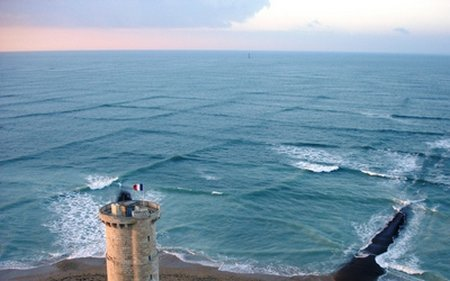
\includegraphics[height=0.4\textheight]{images/livekp.jpg}
    \caption{KP waves off the coast of \^{I}le de R\'{e}, France.}
  \end{figure}
\end{frame}

\begin{frame}{Theta Function Solutions}{}
  KP admits a (large) family of solutions of the form
  \[
  u(x,y,t) = 2 \partial_x^2 \log
  \theta(Ux + Vy + Wt + z_0, \Omega)
  \]
  Where, for any $g \in \ZZ_+$,
  \begin{itemize}
    \item $U,V,W,z_0 \in \CC^g$,
    \item $\Omega \in \CC^{g \times g}$,
    \item $\theta : \CC^g \times \CC^{g \times g} \to \CC$
      is the {\it``Riemann theta function''}.
  \end{itemize}

  \vspace{20pt}

  \begin{block}
  {\it In fact, Theta function solutions are \underline{dense} in the
    space of periodic solutions to KP.}
  \end{block}
\end{frame}

\begin{frame}{Theta Function Solutions}
  The Riemann theta function $\theta:\CC^g \times \CC^{g \times g} \to
  \CC$
  \[
  \theta(z,\Omega) = \sum_{n \in \ZZ^g}
  e^{
    2 \pi i
    \left( \tfrac{1}{2} n \cdot \Omega n + n \cdot z \right)
  }
  \]
  \begin{block}{Convergence}
    $\im(\Omega)$ must be positive definite. Additionally, we only
    consider symmetric $\Omega$. So called space of ``Riemann
    matrices'': $\hh_g$.
  \end{block}
  \[
    \theta:\CC^g \times \hh_g \to \CC
  \]
\end{frame}

\begin{frame}{Demo}{}
  \begin{center}
    Demo: Riemann theta functions.
  \end{center}
\end{frame}



%------------------------------------------------------------------------------
\subsection{Connections to Algebraic Geometry}
%------------------------------------------------------------------------------



\begin{frame}{Connections to Algebraic Geometry}{}
  \[
    \text{KP:} \quad u(x,y,t) = 2 \partial_x^2 \log
    \theta(Ux + Vy + Wt + z_0, \Omega)
  \]
  The constants $U,V,W,z_0,\Omega$ are not arbitrary. They come from a
  ``complex algebraic curve'': given a polynomial $f(X,Y) \in
  \mathbb{C}[X,Y]$
  \[
  F(X,Y) = a_d(X)Y^d + a_{d-1}(X)Y^{d-1} + \cdots + a_0(X)
  \]
  the curve $\Gamma$ is the set
  \[
  \Gamma = \left\{ (X,Y) \in \CC^2 \, : \, F(X,Y) = 0 \right\}.
  \]

  \begin{block}
  {This talk: where does the Riemann matrix $\Omega$ come from and how
    do we compute it?}
  \end{block}
\end{frame}

\begin{frame}{A Simple Example}{}
\end{frame}



%%%%%%%%%%%%%%%%%%%%%%%%%%%%%%%%%%%%%%%%%%%%%%%%%%%%%%%%%%%%%%%%%%%%%%%%%%%%%%%
\section{Computing on Riemann Surfaces}
%%%%%%%%%%%%%%%%%%%%%%%%%%%%%%%%%%%%%%%%%%%%%%%%%%%%%%%%%%%%%%%%%%%%%%%%%%%%%%%

%------------------------------------------------------------------------------
\subsection{Algebra}
%------------------------------------------------------------------------------

\begin{frame}{Holomorphic Differentials}
  Holomorphic Differentials
\end{frame}

%------------------------------------------------------------------------------
\subsection{Geometry}
%------------------------------------------------------------------------------

\begin{frame}{Monodromy}
  Monodromy
\end{frame}

%------------------------------------------------------------------------------
\subsection{{\tt abelfunctions}}
%------------------------------------------------------------------------------

\begin{frame}{{\tt abelfunctions}}
  abelfunctions
\end{frame}


%%%%%%%%%%%%%%%%%%%%%%%%%%%%%%%%%%%%%%%%%%%%%%%%%%%%%%%%%%%%%%%%%%%%%%%%%%%%%%%
\section{Future Work and Applications}
%%%%%%%%%%%%%%%%%%%%%%%%%%%%%%%%%%%%%%%%%%%%%%%%%%%%%%%%%%%%%%%%%%%%%%%%%%%%%%%

\begin{frame}{Schottky Problem}{}
  Counting Riemann matrices $\Omega = X + iY$.
  \begin{itemize}
    \item In general: $g(g+1)/2$ free parameters.
    \item Period Matrices: $3g-3$ free parameters.
  \end{itemize}

  Q: {\it ``For $g \geq 3$, when is a Riemann matrix $\Omega$ a period
    matrix?}

  A: When $u(x,y,t) = 2 \partial^2_x \log \theta(z,\Omega)$ solves the
  KP Equation.
\end{frame}


\begin{frame}[plain,noframenumbering]
  \finalpage{
    {\huge Thank you!} \\
    \vspace{20pt}{\tt \scriptsize cswiercz@uw.edu} \\
    {\tt \scriptsize https://github.com/cswiercz/abelfunctions}
    {\tt \scriptsize https://github.com/cswiercz/general-exam}
  }
\end{frame}

\end{document}
